% Options for packages loaded elsewhere
\PassOptionsToPackage{unicode}{hyperref}
\PassOptionsToPackage{hyphens}{url}
%
\documentclass[
  english,
  man,mask,floatsintext]{apa7}
\usepackage{lmodern}
\usepackage{amssymb,amsmath}
\usepackage{ifxetex,ifluatex}
\ifnum 0\ifxetex 1\fi\ifluatex 1\fi=0 % if pdftex
  \usepackage[T1]{fontenc}
  \usepackage[utf8]{inputenc}
  \usepackage{textcomp} % provide euro and other symbols
\else % if luatex or xetex
  \usepackage{unicode-math}
  \defaultfontfeatures{Scale=MatchLowercase}
  \defaultfontfeatures[\rmfamily]{Ligatures=TeX,Scale=1}
\fi
% Use upquote if available, for straight quotes in verbatim environments
\IfFileExists{upquote.sty}{\usepackage{upquote}}{}
\IfFileExists{microtype.sty}{% use microtype if available
  \usepackage[]{microtype}
  \UseMicrotypeSet[protrusion]{basicmath} % disable protrusion for tt fonts
}{}
\makeatletter
\@ifundefined{KOMAClassName}{% if non-KOMA class
  \IfFileExists{parskip.sty}{%
    \usepackage{parskip}
  }{% else
    \setlength{\parindent}{0pt}
    \setlength{\parskip}{6pt plus 2pt minus 1pt}}
}{% if KOMA class
  \KOMAoptions{parskip=half}}
\makeatother
\usepackage{xcolor}
\IfFileExists{xurl.sty}{\usepackage{xurl}}{} % add URL line breaks if available
\IfFileExists{bookmark.sty}{\usepackage{bookmark}}{\usepackage{hyperref}}
\hypersetup{
  pdftitle={Modelling disfluencies in copy-typing},
  pdflang={en-EN},
  pdfkeywords={Copy-task; keystroke modelling; autoregression; mixture models; Bayesian statistical models; typing skills},
  hidelinks,
  pdfcreator={LaTeX via pandoc}}
\urlstyle{same} % disable monospaced font for URLs
\usepackage{graphicx}
\makeatletter
\def\maxwidth{\ifdim\Gin@nat@width>\linewidth\linewidth\else\Gin@nat@width\fi}
\def\maxheight{\ifdim\Gin@nat@height>\textheight\textheight\else\Gin@nat@height\fi}
\makeatother
% Scale images if necessary, so that they will not overflow the page
% margins by default, and it is still possible to overwrite the defaults
% using explicit options in \includegraphics[width, height, ...]{}
\setkeys{Gin}{width=\maxwidth,height=\maxheight,keepaspectratio}
% Set default figure placement to htbp
\makeatletter
\def\fps@figure{htbp}
\makeatother
\setlength{\emergencystretch}{3em} % prevent overfull lines
\providecommand{\tightlist}{%
  \setlength{\itemsep}{0pt}\setlength{\parskip}{0pt}}
\setcounter{secnumdepth}{-\maxdimen} % remove section numbering
% Make \paragraph and \subparagraph free-standing
\ifx\paragraph\undefined\else
  \let\oldparagraph\paragraph
  \renewcommand{\paragraph}[1]{\oldparagraph{#1}\mbox{}}
\fi
\ifx\subparagraph\undefined\else
  \let\oldsubparagraph\subparagraph
  \renewcommand{\subparagraph}[1]{\oldsubparagraph{#1}\mbox{}}
\fi
% Manuscript styling
\usepackage{upgreek}
\captionsetup{font=singlespacing,justification=justified}

% Table formatting
\usepackage{longtable}
\usepackage{lscape}
% \usepackage[counterclockwise]{rotating}   % Landscape page setup for large tables
\usepackage{multirow}		% Table styling
\usepackage{tabularx}		% Control Column width
\usepackage[flushleft]{threeparttable}	% Allows for three part tables with a specified notes section
\usepackage{threeparttablex}            % Lets threeparttable work with longtable

% Create new environments so endfloat can handle them
% \newenvironment{ltable}
%   {\begin{landscape}\begin{center}\begin{threeparttable}}
%   {\end{threeparttable}\end{center}\end{landscape}}
\newenvironment{lltable}{\begin{landscape}\begin{center}\begin{ThreePartTable}}{\end{ThreePartTable}\end{center}\end{landscape}}

% Enables adjusting longtable caption width to table width
% Solution found at http://golatex.de/longtable-mit-caption-so-breit-wie-die-tabelle-t15767.html
\makeatletter
\newcommand\LastLTentrywidth{1em}
\newlength\longtablewidth
\setlength{\longtablewidth}{1in}
\newcommand{\getlongtablewidth}{\begingroup \ifcsname LT@\roman{LT@tables}\endcsname \global\longtablewidth=0pt \renewcommand{\LT@entry}[2]{\global\advance\longtablewidth by ##2\relax\gdef\LastLTentrywidth{##2}}\@nameuse{LT@\roman{LT@tables}} \fi \endgroup}

% \setlength{\parindent}{0.5in}
% \setlength{\parskip}{0pt plus 0pt minus 0pt}

% \usepackage{etoolbox}
\makeatletter
\patchcmd{\HyOrg@maketitle}
  {\section{\normalfont\normalsize\abstractname}}
  {\section*{\normalfont\normalsize\abstractname}}
  {}{\typeout{Failed to patch abstract.}}
\makeatother
\shorttitle{Modelling disfluencies in copy-typing}
\author{Jens Roeser\textsuperscript{1}, Sven De Maeyer\textsuperscript{2}, Mariëlle Leijten\textsuperscript{3}, Mark Torrance\textsuperscript{1}, \& Luuk Van Waes\textsuperscript{3}}
\affiliation{
\vspace{0.5cm}
\textsuperscript{1} Department of Psychology, Nottingham Trent University, United Kingdom\\\textsuperscript{2} Faculty of Social Sciences, University of Antwerp, Belgium\\\textsuperscript{3} Department of Management, University of Antwerp, Belgium}
\authornote{

Correspondence concerning this article should be addressed to Jens Roeser, 50 Shakespeare St, Nottingham NG1 4FQ. E-mail: jens.roeser@ntu.ac.uk}
\keywords{Copy-task; keystroke modelling; autoregression; mixture models; Bayesian statistical models; typing skills}
\usepackage{csquotes}
\usepackage{booktabs}
\usepackage{longtable}
\usepackage{array}
\usepackage{multirow}
\usepackage{float}
\usepackage{colortbl}
\usepackage{threeparttable}
\usepackage[normalem]{ulem}
\usepackage[utf8]{inputenc}
\usepackage{icomma}
\ifxetex
  % Load polyglossia as late as possible: uses bidi with RTL langages (e.g. Hebrew, Arabic)
  \usepackage{polyglossia}
  \setmainlanguage[]{english}
\else
  \usepackage[shorthands=off,main=english]{babel}
\fi
\ifluatex
  \usepackage{selnolig}  % disable illegal ligatures
\fi
\newlength{\cslhangindent}
\setlength{\cslhangindent}{1.5em}
\newenvironment{cslreferences}%
  {\setlength{\parindent}{0pt}%
  \everypar{\setlength{\hangindent}{\cslhangindent}}\ignorespaces}%
  {\par}

\title{Modelling disfluencies in copy-typing}

\date{}

\abstract{
The analysis of keystroke latency data typically involves the calculation of summary statistics such as the mean inter-keystroke interval, pause frequencies etc. There are two fundamental problems with this: first, summary statistics ignore important information in the data and frequently result in biased estimates; second, pauses and pause-related measures are defined using threshold values which are, in principle, arbitrary. We implemented a series of Bayesian models that aimed to address both issues by providing reliable estimates for individual typing speed and statistically inferred process disfluencies. We tested these models on a random sample of 250 participants from the Dutch copy-task corpus. Our results illustrate that process disfluencies can be statistically captured as a mixture process of fluent and disfluent typing. Mixture models provide a principled approach to detect disfluencies in keyboard typing data.
}

\begin{document}
\maketitle

\hypertarget{introduction}{%
\section{Introduction}\label{introduction}}

Writing research has made extensive use of keystroke-logging to capture typing process data. In particular process disfluencies (loosely defined as relatively long intervals between subsequent keystrokes) are interesting to develop an understanding of an individuals writing progress. This is because language production is typically thought of as a cascade from the mental generation of a message, into grammatical processing and finally the generation and execution of motor codes that serve the transmission of an idea. This can be found in theoretical models of speech (Bock \& Ferreira, 2014), handwriting (Van Galen, 1991) and keyboard typing (Hayes, 2012). Disfluencies at the execution stage are therefore indicators of process demands that arise on higher levels of mental representation (Christiansen \& Chater, 2016; Olive, 2014); for example when preplanning syntactic dependencies (Roeser, Torrance, \& Baguley, 2019) or retrieving the lexical entry of a word or its spelling (Torrance, Rønneberg, Johansson, \& Uppstad, 2016). At present there is no principled way for detecting keystroke lags that can be considered a process disfluency. In this paper we present a series of statistical models that aim to capture process disfluencies and produce individual estimates of typing performance.

Keystroke logs provide rich information about the typing process. From these log, researchers can calculate different process measures including measures of writing fluency (Chukharev-Hudilainen, Saricaoglu, Torrance, \& Feng, 2019; Medimorec \& Risko, 2016; Medimorec, Young, \& Risko, 2017; Van Waes \& Leijten, 2015). To name a few, researchers have performed data analysis on means, medians and standard deviations (SD) of inter-keystroke intervals (the latency between two consecutive keystrokes), number of pauses or pause duration and within-word keystroke intervals (for an overview of frequently used keystroke measures see Conijn et al., 2019a). Conijn et al. (2019a) suggested that these aggregates are sensitive to processing difficulty that arises on different levels of mental representation. However, there are two substantial problems tight to the use summary statistics to develop an understanding of the typing process.

First, pause frequencies, writing bursts and related measures are used to assess writing performance (e.g.~Alves \& Limpo, 2015; Beers, Mickail, Abbott, \& Berninger, 2017; Zhang, Bennett, Deane, \& Rijn, 2019). These measures require a definition of what passes as a pause (Van Waes, Leijten, Lindgren, \& Wengelin, 2016; Wengelin, 2006), i.e.~a pause criterion threshold often set to 2 secs (Chanquoy, Foulin, \& Fayol, 1996; Kaufer, Hayes, \& Flower, 1986; Sullivan \& Lindgren, 2002; Wengelin, 2002) or some other lower bound (Chukharev-Khudilaynen, 2014; Connelly, Dockrell, Walter, \& Critten, 2012; Leijten \& Van Waes, 2013). Researchers have stipulated pause thresholds specific to their research purposes and based on prior research. However, ideally, this threshold would need to be specific to both the writing task and the skills of the typist (Wengelin, 2006). For example, when comparing the frequency of pauses larger than 2 secs for a dyslexic and a normal typist, one might observe more pauses for the dyslexic because 2 secs are indeed not unusual transitions between two keystrokes for a dyslexic writer or pauses for the normal typist are typically shorter than 2 secs and therefore unobserved given a 2 secs pause criterion (Wengelin, 2001). This bias would also affect the interpretation of results from L2 typists and other threshold criteria (Van Waes \& Leijten, 2015).

Second, data aggregation results in the loss of important information about disfluencies and time course variation. Even if this variation is not of interest to a research question, parametric aggregates such as mean and SD, and even non-parametric descriptives such as median and IQR, are biased estimates. This is because mean and median are representative for the centre of a normal distribution but keystroke intervals are non-normal distributed as they are zero-bound and therefore right-skewed.\footnote{In fact, the minimum size of keystroke intervals is a function of the time it takes to plan and execute the motor program and keyboard polling.} Therefore, data aggregation may lead to incorrect inference based on biased parameter values (Baaijen \& Galbraith, 2018). To prevent biased parameter values researchers used data transformation and data trimming (Hoaglin \& Iglewicz, 1987) to remove data that were \emph{a priori} considered outliers. The removal of such values will inevitably impact differently on struggling writers and normal writers, skew the resulting typing estimates and therefore potentially the conclusions drawn from the data.

A central methodological challenge with implications for writing research (Hayes, 2012; Kaufer et al., 1986; Van Waes et al., 2016; Wengelin, 2006) is the detection of writing disfluencies. We addressed this problem by implementing statistical models that aim to capture the nature of the data generating process (i.e.~keyboard typing). Crucially we want these models to provide reliable estimates of typing performance without subjecting the data to trimming and threshold criteria, aggregation or manual manipulation.

\hypertarget{modelling-typing-process-data}{%
\section{Modelling typing process data}\label{modelling-typing-process-data}}

As a guiding principle, we aim to produce statistical models that represent the assumed mental process that generates the data. Keystrokes are the end of a cascade of mental processes. The lags between subsequent keypresses, for example, the transitions c\(^{\wedge}\)a\(^{\wedge}\)t for the word \emph{cat} where \(^{\wedge}\) respectively indicates the inter-keystroke interval (IKI) between pressing \(<\)c\(>\) and \(<\)a\(>\), and \(<\)a\(>\) and \(<\)t\(>\), are therefore symptomatic for process difficult on higher levels of activation. These keystroke intervals reflect at minimum two states of the information flow; either information flows or the flow is being inhibited. Inhibition is then resulting in process disfluencies expressed in a larger lag between subsequent keys. Our models should provide a systematic way of addressing process disfluencies; e.g.~when the lag before pressing \(<\)a\(>\) is unusually large. We implemented a series of models for keystroke. The quality of fit of these models is compared in the Results section.

Statistical models can be used to characterize the underlying data generating process as a function of parameter values. For example, if we assume that there is a single underlying process that generates normal distributed data, we can discribe this process with a mean \(\mu\) and a variance \(\sigma^2\). The values of the parameters \(\mu\) and \(\sigma^2\) are unknown and typically used to represent task and populations specific (typing) performance. The model of the data can be written as \(y \sim Normal(\mu, \sigma^2)\); i.e.~the data \(y\) come from a single process that follows a normal distribution with an unknown mean \(\mu\) and an unknown error variance \(\sigma^2\). Our statistical model will then determine values for these parameters that can be considered reliable if the data satisfy the model assumption; i.e.~the data come from a single process that generates normal distributed data.

Bayesian models, as used in this paper, are ideal for a reliable estimation of the parameter values of interest expressed in probability distribution (Farrell \& Lewandowsky, 2018; Gelman et al., 2014; Lee \& Wagenmakers, 2014). To achieve this, Bayesian models require the explicit inclusion of prior information, i.e.~existing knowledge about parameter values. For small data sets non-uninformative priors influence the posterior (inferred parameter estimates) but for larger data sets the prior is quickly overcome by the data (i.e.~automatic Ockam's razor; Jefferys \& Berger, 1992) so that the choice of priors (reflecting existing knowledge) impacts the posterior to a lesser extent. In the present paper, priors are used to aid model convergence by constraining the parameter space (i.e.~using weakly regulating priors; Lambert, 2018; McElreath, 2016).

We assume throughout that IKIs can be characterized as log-normal distributed because IKIs are zero-bound (Baayen, 2008). To be able to estimate the parameter of interests, e.g.~the mean \(\mu\), we need a model that accounts for other sources of variance. This can be achieved with linear mixed-effects models (LMM) which have been used to model keystroke data (Leijten, De Maeyer, \& Van Waes, 2011; Quené \& Van den Bergh, 2004; Van Waes, Leijten, \& Quinlan, 2010; Van Waes, Leijten, Roeser, Olive, \& Grabowski, 2020). The LMM in equation \ref{eq:lmm} is an extension of the simple example above. Sources of random error variance in this model are participants \(u\) and keystroke bigrams \(w\).

\[
\tag{1}
\begin{aligned}
y_{ij} \sim LogNormal(\mu + u_i + w_j, \sigma_e^2)\\
\end{aligned}
\label{eq:lmm}
\]

We know that some participants are faster typists than other participants and some bigrams are easier to type than others. Differences associated with participant \(i\), expressed as \(u_i\), can be assumed to be normal distributed around 0 with a between participants variance \(\sigma_u^2\) with \(i = 1, \dots, I\), where \(I\) is the number of participants (see \ref{eq:lmm2}). The variance \(\sigma_u^2\) is given a half-Normal prior (because a variance is never negative) with a mean of 0 and a variance of 2.5 (see e.g.~Sorensen, Hohenstein, \& Vasishth, 2016).

\[
\tag{2}
\begin{aligned}
u_i \sim Normal(0,\sigma_u^2)\\
\sigma_u \sim Normal(0,2.5)\\
\text{constraint: } \sigma_u >0 
\end{aligned}
\label{eq:lmm2}
\]

Variation between keystroke pairs (i.e.~letter bigrams) \(w\) is added as random intercepts term in equation \ref{eq:lmm} (Van Waes, Leijten, Pauwaert, \& Van Horenbeeck, 2019; Van Waes et al., 2020). More specifically, this is to assume that each bigram \(j\) with \(j = 1, \dots, J\), where \(J\) is the total number of bigrams, is independent of the other bigrams. Each bigram intercept difference \(w_j\) is distributed around 0 with a between bigram variance \(\sigma_w^2\) (equation \ref{eq:lmm5}).

\[
\tag{3}
\begin{aligned}
w_j \sim Normal(0,\sigma_w^2)\\
\sigma_w \sim Normal(0,2.5)\\
\text{constraint: }\sigma_w >0 
\end{aligned}
\label{eq:lmm5}
\]

In other words, the parameter estimate for the mean \(\mu\) in equation \ref{eq:lmm} is the marginalised value after taking into account random variation between participants \(u\) and bigrams \(w\). To aid efficient sampling, we parameterised the mean \(\mu\) as non-centred in all models with regulating priors (equation \ref{eq:lmm3}; following Gelman et al., 2014).

\[
\tag{4}
\begin{aligned}
\mu = \alpha_{\mu} + \sigma_{\mu} \cdot \epsilon\\
\alpha_{\mu} \sim Normal(5,2)\\
\sigma_{\mu} \sim Normal(0,1)\\
\epsilon \sim Normal(0,1)\\
\text{constraint: }\mu_{\sigma}>0 
\end{aligned}
\label{eq:lmm3}
\]

For the unexplained variance \(\sigma_e^2\) we used an uninformative half-Cauchy prior (equation \ref{eq:lmm4}; see Gelman et al., 2014).

\[
\tag{5}
\begin{aligned}
\sigma_e \sim Cauchy(0,2.5)\\
\text{constraint: }\sigma_e>0 
\end{aligned}
\label{eq:lmm4}
\]

\hypertarget{typing-as-autoregressive-process}{%
\subsection{Typing as autoregressive process}\label{typing-as-autoregressive-process}}

The previous model captures variation associated with particular bigrams but assumes that disfluencies are subject to random noise. Further, this analysis assumes that subsequent keystrokes are independent and thus exchangeable. IKIs are not necessarily independent; IKI\(_{i}\) might be related to IKI\(_{i-1}\) preceding it (Conijn et al., 2019b). In other words, we can predict an IKI with the previous keystroke and capture their relationship with a parameter \(\phi\); see equation \ref{eq:ark}. This is called an autoregressive process (Eltahir, Salami, Ismail, \& Lai, 2004). This model captures disfluencies as slowdown relative to a previous keystroke. The autocorrelation was assumed to vary for each participant \(\phi_i\) with a centred mean \(\mu_{\phi}\) and error variance \(\eta^2\).

\[
\tag{6}
\begin{aligned}
y_{ij} \sim LogNormal(\mu + \phi_i*log(y_{ij-1}) + u_i, \sigma_e^2)\\
\text{where}\\
\phi_i \sim Normal(\mu_{\phi}, \eta^2)\\
\mu_{\phi} \sim Normal(0, 1)\\
\eta \sim Cauchy(0, 1)\\
\text{constraint: }\eta >0 
\end{aligned}
\label{eq:ark}
\]

\hypertarget{typing-as-mixture-process}{%
\subsection{Typing as mixture process}\label{typing-as-mixture-process}}

Alternatively, we can capture process disfluencies using a finite-mixture model (e.g.~Farrell \& Lewandowsky, 2018; Gelman et al., 2014). Mixture models allow us to model data as coming from a combination of processes (see e.g.~Vasishth, Chopin, Ryder, \& Nicenboim, 2017; Vasishth, Jäger, \& Nicenboim, 2017). For the present purposes we constrain the model to be finite. In particular, we assume that the data map onto a mixture of two processes; information flow into keystrokes is either inhibited or not. This inhibition has an unknown probability. In other words, we fixed the number of underlying distributions to two, namely 2 log-Gaussian (normal) distributions, of which one represents fluent typing (shorter IKIs) and the other represents disfluencies (longer IKIs). This model can be summarised as in equation \ref{eq:mog}, following Vasishth et al. (2017). The first and second line represent that the data \(y\) are modelled as the sum of two weighted log-normal distributions of which the first distribution has a mixing proportion \(\theta\) and the other distribution receives the remaining proportion \(1-\theta\). Both distributions have the same mean \(\mu\). The parameter \(\delta\), constrained to be positive, was added to the first distribution to capture the latency magnitude of process disfluencies with \(\theta\) indicating the probability of disfluencies to occur. The probability of disfluent IKIs \(\theta_i\) was allowed to vary across participants \(i\) because the probability to exhibit disfluencies can be assumed to depend on individual typing style (skills).

\[
\tag{7}
\begin{aligned}
    y_{ij} \sim \theta_i \cdot LogNormal(\mu + \delta + u_i + w_j, \sigma_{e'}^2) +\\
        (1 - \theta_i) \cdot LogNormal(\mu + u_i + w_j, \sigma_{e}^2)\\
        \text{where}\\
        \delta \sim Normal(0,1)\\
        \text{constraint: } \delta > 0
\end{aligned}   
\label{eq:mog}
\]

As shown in equation \ref{eq:mog2}, a continuous prior was placed on the logit of the individual mixing proportions \(\alpha_i\), which was transformed to a proportion, using the inverse-logit function, to range between 0 to 1, and stored in \(\theta_i\). We used a normal prior for the logit of individual mixing proportions \(\alpha_i\) with a mean \(\mu_{\alpha}\) that captures the logit of the population disfluency probability (with an error variance \(\tau^2\)). The hyper-prior on the population mixing-proportion \(\mu_{\alpha}\) was assumed to have a mean of logit 0, corrsponding to a probability of 0.5 and a variance of logit 1 (i.e.~\(\approx\) 0.73 in proportion).

\[
\tag{8}
\begin{aligned}
        \theta_i = Logit^{-1}(\alpha_i)\\
        \alpha_i \sim Normal(\mu_{\alpha},\tau^2)\\
        \mu_{\alpha} \sim Normal(0,1)\\
        \tau \sim Cauchy(0,1)\\
        \text{constraint: } \tau > 0
\end{aligned}   
\label{eq:mog2}
\]

As longer latencies are known to be associated with a larger variances for both response-time data in particular (Wagenmakers \& Brown, 2007) and human motor behaviour in general (Schöner, 2002; Wing \& Kristofferson, 1973), the variance \(\sigma_{e'}^2\) associated with the distribution of typing disfluencies was constrained to be larger than the variance for normal typing \(\sigma_e^2\) as shown in \ref{eq:mog3} (see Vasishth et al., 2017; Vasishth et al., 2017).

\[
\tag{9}
\begin{aligned}
        \sigma_{e'} = \sigma + \sigma_{\text{diff}}\\
        \sigma_{e} = \sigma - \sigma_{\text{diff}}\\
        \sigma_{\text{diff}} \sim Normal(0,1)\\
        \sigma \sim Cauchy(0,2.5)\\
        \text{constraint: } \sigma, \sigma_{\text{diff}}, \sigma_{e'}, \sigma_{e} > 0
\end{aligned}   
\label{eq:mog3}
\]

\hypertarget{typing-as-autoregressive-mixture-process}{%
\subsection{Typing as autoregressive mixture process}\label{typing-as-autoregressive-mixture-process}}

The mixture model, as well as the LMM, assume that lags between subsequent letter bigrams are independent of each other. This is likely to be the case for an IKI that follows a disfluency. However IKIs in fluent typing might involve some autocorrelation. Therefore, we implemented another mixture model but replaced random bigram intercepts \(w_j\) in the distribution that represents fluent typing, see equation \ref{eq:mog}, with an autoregressor \(\phi_i*y_{ij-1}\), as in equation \ref{eq:ark}; random bigram intercepts were kept for the distribution of disfluent typing intervals.

\hypertarget{method}{%
\section{Method}\label{method}}

To test which model captures the typing process best, we applied a series of models as described in the previous section to data from a subset of the Dutch copy-task corpus (Leijten \& Van Waes, 2013; Van Waes et al., 2019; Van Waes et al., 2020). An overview of all models can be found in Table \ref{tab:models}.

\begin{table}[!ht]

\begin{center}
\begin{threeparttable}

\caption{\label{tab:models}Overview of typing process models. All models were fitted with random intercepts for participants.}

\begin{tabular}{llll}
\toprule
Models & \multicolumn{1}{c}{Type} & \multicolumn{1}{c}{Equation} & \multicolumn{1}{c}{Description}\\
\midrule
M1 & LMM & \ref{eq:lmm} & Random intercepts for bigram order\\
M2 & AR & \ref{eq:ark} & Autocorrelation between subsequent IKIs\\
M3 & MoG & \ref{eq:mog} & Mixture process of normal and disfluent typing\\
M4 & AR + MoG &  & As M3 but autocorrelation for normal typing\\
\bottomrule
\addlinespace
\end{tabular}

\begin{tablenotes}[para]
\normalsize{\textit{Note.} LMM = Linear mixed-effects models; AR = Autoregressive model; MoG = Mixture of log-Gaussians}
\end{tablenotes}

\end{threeparttable}
\end{center}

\end{table}

The copy-task corpus consists of keystroke data collected via Inputlog, a Javascript-based web application available on \url{www.inputlog.net} with the source code released on \href{https://github.com/lvanwaes/Inputlog-Copy-Task}{github.com/lvanwaes/Inputlog-Copy-Task} and \href{https://zenodo.org/record/2908966}{zenodo.org/record/2908966}. In a set of different subtasks participants have to produce keyboard typed responses. In this analysis we focus on the consonants task and the low-frequency (LF) bigrams task. In the consonant task, participants saw and copy-typed a single time four blocks of six consonant sequences; i.e.~``tjxgfl pgkfkq dtdrgt npwdvf''. This task allows us to measure typing skills in a non-linguistic environment (Grabowski, Weinzierl, \& Schmitt, 2010). We repeated the analysis for the LF-bigrams task to contrast the non-lexical consonants task with a lexical copy task. In the LF-bigram task, participants typed three-word combinations seven times (\emph{een chaotische cowboy} `a chaotic cowboy' in the Dutch version) of which four bigrams are low frequent. For comparability to the consonant task, we used the data from all bigrams but removed all repetitions after the first time the three-word sequence was copied. Importantly for the present purpose, fluent copying and pausing may be thought of as a function (1) the complexity to the letter sequences and (2) the participant's memory span and typing skill; for example touch-typists may depend less on memory representation of the to-be typed bigrams for fluent copying than hunt-and-peck typists. This results in a combination of fluent typing and typing interruptions. In other words, for these task we need to be able to disentangle fluent and disfluent IKIs. We used a random sample of 250 participants (178 females, 69 males, 3 unknown) from the age range of 18 to 25 years (median age = 22 years). Before analysis we excluded spaces and editing operations from the data.

\hypertarget{results}{%
\section{Results}\label{results}}

\hypertarget{data-overview}{%
\subsection{Data overview}\label{data-overview}}

The IKI data for the LF-bigrams task and the consonants task are visualized in Figure \ref{fig:descriptives}. In the upper panels of the LF-bigrams data and the consonants data in Figure \ref{fig:descriptives}A the data are visualised for each participant. In the respective lower panels of Figure \ref{fig:descriptives}A, different measures of central tendency are shown; and repeated for the IKI density functions in Figure \ref{fig:descriptives}B.

\begin{figure}[!ht]

{\centering 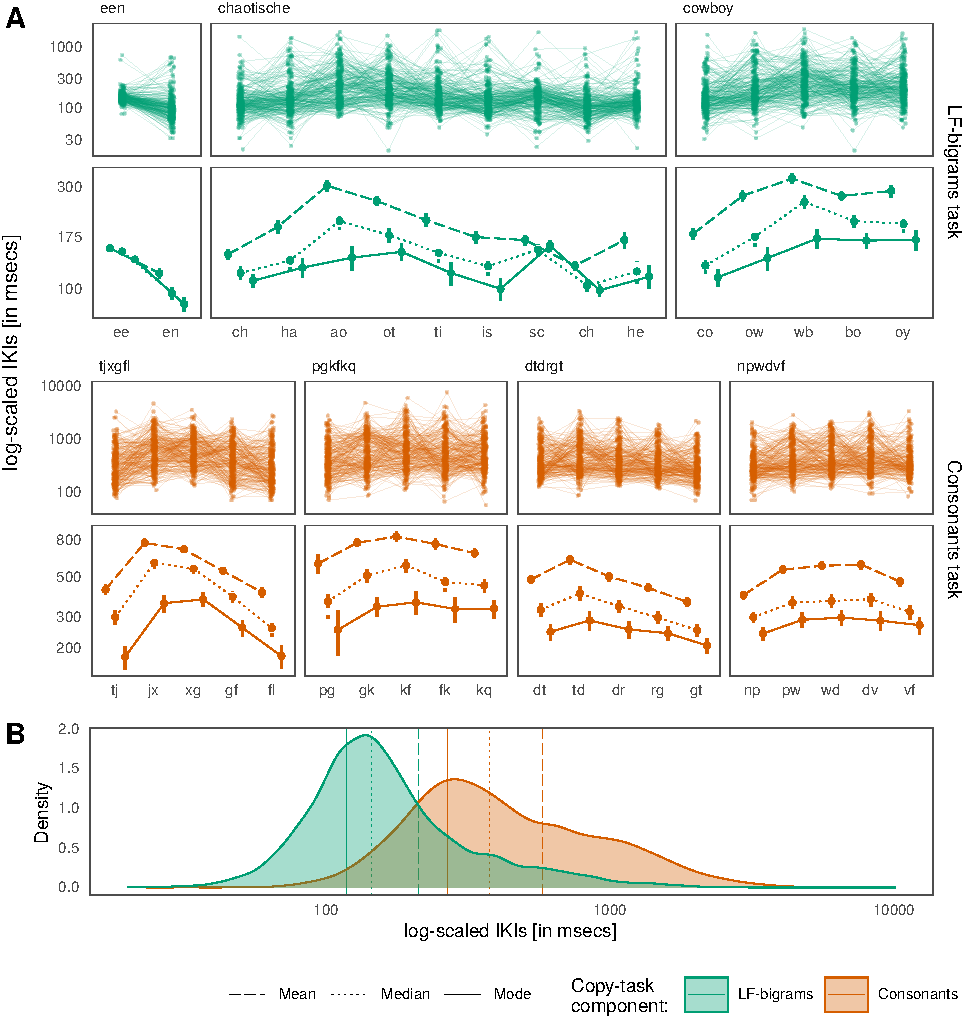
\includegraphics{report_files/figure-latex/descriptives-1} 

}

\caption{Data overview. Panel A illustrates IKIs over bigrams position (time course) by participant in the upper rows and as different measures of central tendency (with standard error [SE]) in the lower rows for each the LF-bigrams task and the consonants task. Panel B shows the density distribution of IKI data with the same central tendency descriptors as in panel A.}\label{fig:descriptives}
\end{figure}

These visualisation highlight two important points: (1) aggregating data neglects individual time-course variability in the data; (2) the choice of central tendency measure might lead to different conclusions about patterns in the data. As for the first point, Figure \ref{fig:descriptives}A shows that participants slow down and speed up throughout the trial but do not show consistent patterns for the same letter bigrams as suggested in the corresponding summary statistics. Central tendency measures in the lower panels of Figure \ref{fig:descriptives}A suggest that some slowdowns and speedups might be bigram specific if we disregard by-participant variability. For example, in the LF-bigrams task, the first bigram is followed by a faster IKI; in the consonant task, the first bigram is followed by a slowdown. Importantly though, there is a substantial variability between participants.

As for the second point, the choice of central-tendency measure might affect whether we consider an observation a disfluency, or a participant to be prone to disfluent typing. In particular, means are systematically longer than the median and mode. Figure \ref{fig:descriptives}B illustrates why this is the case. Shown are the density functions for the LF-bigrams and the consonants task. Even log-scaled data show skewed distributions with a heavy right tail. While in a normal distribution the mean, median and mode have identical values, the conceptual differences between these three measures of central tendency lead to different values in non-normal distributed data. In particular, means are known to be sensitive to extreme values. Extreme values are inevitable as IKIs are zero-bound but have, in principle, no upper bound. Thus, on a participant level, large means might be the consequence of a few larger IKIs that over-shadow largely normal typing behaviour. Means are closer to the horizontal middle of the data space which, for right-skewed distributions, is on the right of the distribution's peak (the value with the highest kernel density). The latter is being represented by the mode. Regardless of which measure is uesd, all three central tendency indicators ignore important properties of the distribution. That is, measures of central tendency neglect the variability in the data as illustated in the shown distributions; also keystroke data might indeed represent a combination of processes; e.g.~normal typing and disfluencies. Central tendency measures do not per se allow us to distinguish between IKIs that are the results of fluent typing and IKIs that reflect process lags.

In sum, data aggregation does not just neglect participant-specific typing patterns but the choice of central tendency may affect the conclusions about the data. To ensure accurate statistical inference, we need to be able to account for participant-specific typing patterns as expressed across the typing time-course.

\hypertarget{model-fit}{%
\subsection{Model fit}\label{model-fit}}

All models were implemented as Bayesian models (see e.g.~Gelman et al., 2014; Lambert, 2018; McElreath, 2016) in the probabilistic programming language Stan (Carpenter et al., 2016; Hoffman \& Gelman, 2014; Stan Development Team, 2015a, 2015b). Data, \textit{R}-scripts and \textit{Stan}-code are available on OSF (\href{https://doi.org/10.17605/OSF.IO/Y3P4D}{doi.org/10.17605/OSF.IO/Y3P4D}). Models were fitted with 30,000 iterations (15,000 warm-up) on 3 MCMC chains. Convergence was tested via the Rubin-Gelman statistic (Gelman \& Rubin, 1992), traceplots and cross-validation (Vehtari, Gelman, \& Gabry, 2015, 2017).

The predictive performance of the models was established using leave-one-out cross-validation. Cross-validation penalizes models with more parameters and therefore prevents overfit (see Farrell \& Lewandowsky, 2018; Lambert, 2018; Lee \& Wagenmakers, 2014; McElreath, 2016). The out-of-sample predictive performance was determined via Pareto smoothed importance-sampling (Vehtari et al., 2015, 2017) and estimated as sum of the expected log predictive density (\(\widehat{elpd}\)). \(\widehat{elpd}\) was used to compare the predictive quality of our models. Model comparisons can be found in Table \ref{tab:modelcomparisons}. Model comparisons revealed higher predictive performance for the mixture model M3 for both copy-task components. The differences in predictive performance of the remaining models shows the same pattern in both copy-task components. For the consonants tasks, the combination of mixture and autoregressive-process model as implemented in model M4 revealed a negligibly different predictive performance compared to the mixture model M3 (see equation \ref{eq:mog}). As model M3 is simpler than model M4 but the predictive performance was similar, we preferred model M3 over model M4 for the consonants task. For LF-bigrams task, model M3 showed a higher predictive performance than all other models. We therefore chose model M3 for parameter evaluation of both copy-task components.

\begin{table}[!ht]

\begin{center}
\begin{threeparttable}

\caption{\label{tab:modelcomparisons}Model comparisons expressed as expected log predictive density ($\widehat{elpd}$). The top row of each copy-task component shows the model with the highest predictive performance. Differences in predictive performance are shown as $\Delta\widehat{elpd}$ contrasting for each copy-task component the model in the first row and the remaining models. Standard errors (SE) are shown in brackets.}

\begin{tabular}{lllr}
\toprule
Model & \multicolumn{1}{c}{Type} & \multicolumn{1}{c}{$\Delta\widehat{elpd}$} & \multicolumn{1}{c}{$\widehat{elpd}$}\\
\midrule
Consonants &  &  & \\
\ \ \ M3 & MoG & 0 (0) & -37,069 (101)\\
\ \ \ M4 & AR + MoG & -9 (17) & -37,078 (101)\\
\ \ \ M1 & LMM & -281 (25) & -37,350 (99)\\
\ \ \ M2 & AR & -490 (29) & -37,560 (97)\\
LF bigrams &  &  & \\
\ \ \ M3 & MoG & 0 (0) & -33,178 (113)\\
\ \ \ M4 & AR + MoG & -413 (40) & -33,591 (112)\\
\ \ \ M1 & LMM & -994 (63) & -34,173 (121)\\
\ \ \ M2 & AR & -1,361 (50) & -34,540 (109)\\
\bottomrule
\addlinespace
\end{tabular}

\begin{tablenotes}[para]
\normalsize{\textit{Note.} LMM = Linear mixed-effects models; AR = Autoregressive model; MoG = Mixture of log-Gaussians}
\end{tablenotes}

\end{threeparttable}
\end{center}

\end{table}

The second best performing model, for both copy-task components, is the mixture model M4 with an by-participant autoregressor for fluent typing only. Adding the autoregressor instead of random bigram intercepts for fluent typing did not improve the predictive performance of the mixture model per se. In fact, the autoregressive model was found to be the model with the lowest predictive performance. Modelling bigrams as random intercepts (with and without by-participant slope adjustments) was found to have a higher predictive performance compared to the autoregession model. However a higher predictive performance for M4 suggests that addressing the dependence of subsequent IKIs increases the predictive performance only then, if we limit the autocorrelation assumption to those keystroke transitions that were assumed to be non-disfluent. Alternatively, modelling IKIs as coming from a mixture of fluent typing and process disfluencies might lead to a higher predictive performance regardless of how we treat inter-bigram variations. In fact, this was the case for the consonant-task data reflected in the neglligible differences between mixture model M3 and M4 in consonants-task data but not in the LF-bigrams task data. If the majority of keystroke transitions are disfluent, as we will see in the following for the consonants-task data, we would expect no notable difference between M3 and M4.

\hypertarget{parameter-evaluation}{%
\subsection{Parameter evaluation}\label{parameter-evaluation}}

The copy-typing process as expressed by the mixture model can be characterized with the posterior distributions of the model's parameter values. The process relevant parameters are illustrated in Figure \ref{fig:parameters}. Firstly, the modelled IKIs for fluent typing are shown in Figure \ref{fig:parameters}A. This figure shows the typing speed of each participant after accounting for typing disfluencies. Each horizontal line represents the statistically inferred estimate for a participant in the sample ordered from the fastest to the slowest typist for each copy-task separately. The pooled population estimate for fluent typing is 276 msecs embraced by a 95\% probability interval (PI) with a lower bound of 251 and an upper bound of 302 for the consonants task and 162 msecs (95\% PI: 148, 176) for the LF-bigrams task. Figure \ref{fig:parameters}B shows the disfluency probabilities. This parameter captures, for each participant, the probability to exhibit a typing disfluency. On the population level, the disfluency probability was found to be 0.73 (95\% PI: 0.66, 0.80) for the consonants task and 0.34 (95\% PI: 0.31, 0.38) for the LF-bigrams task. In other words, in the consonants task disfluent keystroke transitions are three times more probable than fluent transitions but in the LF-bigrams task, only one out of three transitions consitutes a disfluency. For each participant the model captures varying pausing probabilities that express individual but also task-specific typing difficulty. Although on the population level disfluencies are more probable for the consonants task this is not the case for all participants (as indicated by individual estimates below 0.5 in Figure \ref{fig:parameters}B indicating a larger probability of fluent keystroke transitions).

\begin{figure}[!ht]

{\centering 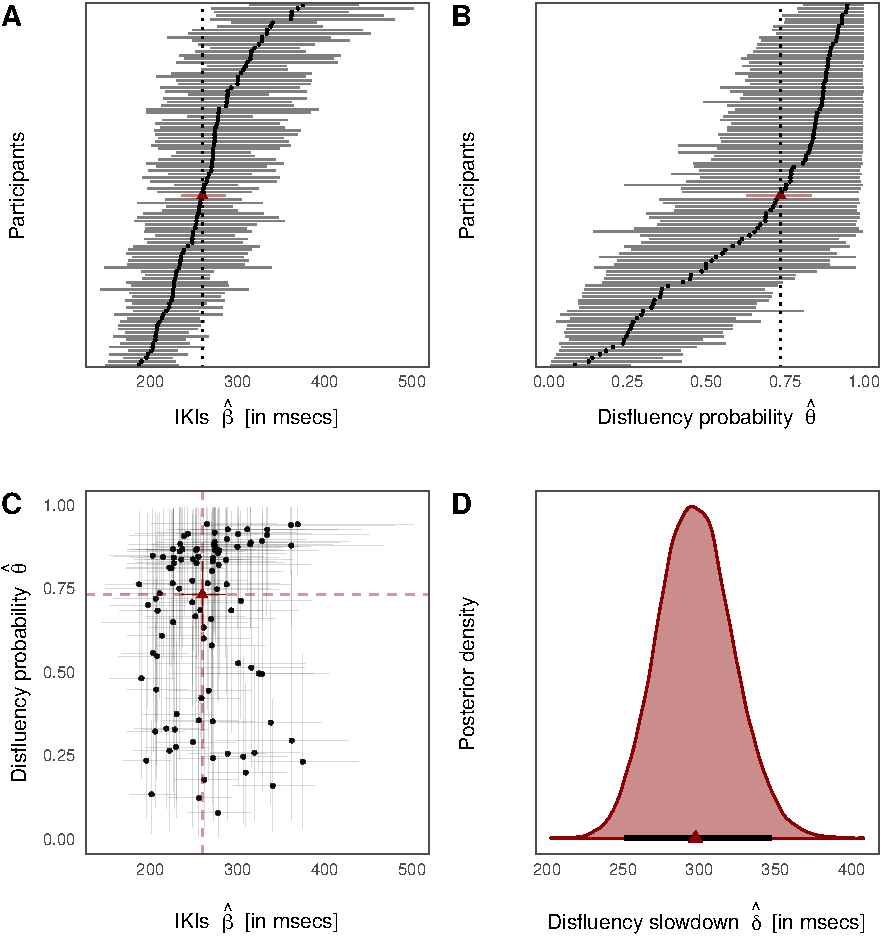
\includegraphics{report_files/figure-latex/parameters-1} 

}

\caption{Parameter values of the mixture models for the LF-bigrams and the consonants task. Panel A shows the infered by-participant IKIs for fluent typing and Panel B shows the disfluency probabilities. Panel C shows estimates for fluent typing plotted against disfluency probability (black symboles indicate overall parameter values). Panel D shows the infered disfluency slowdown. Error bars are 95\% probability intervals.}\label{fig:parameters}
\end{figure}

Values in Figure \ref{fig:parameters}A and Figure \ref{fig:parameters}B are ordered for each task on the basis of the the most probable parameter. In other words, these two figures do not suggest a relationship between individual tpying speed and disfluency probabilities. In Figure \ref{fig:parameters}C we plotted the estimates for individual typing speed against the disfluency probability. Shown are the parameter estimates for each participant and the overall pooled estimates (in black with 95\% PIs). Figure \ref{fig:parameters}C suggests that individual typing speed and pausing disfluency are independent. In other words, fast as well as slow copy-typists show low and high disfluency probabilities. Also, the between-participant variability for both parameters, fluent typing and disfluency probabilities, is larger in the consonants task than in the LF-bigrams task. This suggest that copy-typing strategies used by the participants are more diverse for the consonants task compared to the strategies used for the LF-bigrams task.

Lastly, the inferred slowdown parameter values for disfluent typing are shown in Figure \ref{fig:parameters}D. Disfluent typing was estimated to be 258 msecs (95\% PI: 226, 293) slower than fluent typing in the consonant task and 96 msecs (95\% PI: 79, 115) slower than fluent typing in the LF-bigrams task. In other words, the magnitude for disfluencies in the typing process is task-specific with shorter interruptions for the LF-bigrams task compared to the consonants task.

Faster participants might, in principle, show larger disfluency magnitudes; i.e.~the size of the disfluency magnitude may vary by participant. To test this possibility we implemented two more models that are largly identical to model M3 (see equation \ref{eq:mog}): first, we allowed both the disfluency probability \(\theta\) and the disfluency magnitude \(\delta\) to vary by participant; second, \(\delta\) but not \(\theta\) was allowed to vary by participant. We compared the predictive performance of either model to model M3. Neither model was convincingly better than model M3, neither for the consonants task nor for the LF-bigrams task. For the consonants data, allowing \(\delta\) and \(\theta\) to vary by participant resulted in negligably better predictive performance compared to model M3 (\(\Delta\widehat{elpd}\)=7, SE=4); holding the disfluency probability \(\theta\) constant while allowing the disfluency magnitude \(\delta\) to vary by participant revealed a lower predictive performance (\(\Delta\widehat{elpd}\)=-100, SE=50). The same patterns was found for LF bigrams: allowing \(\delta\) to vary rendered no predictive gain (\(\Delta\widehat{elpd}\)=-1, SE=0.50); fixing \(\theta\) and allowing \(\delta\) to vary showed a decrease in predictive performance (\(\Delta\widehat{elpd}\)=-30, SE=8).

Overall, the values of the three process-central model parameters -- fluent typing speed, disfluency probability, and slowdown magnitude for disfluencies -- were found to be task sensitiv. The LF-bigrams task shows shorter typing intervals, a lower disfluency probability compared to the consonant task and a shorter slowdown magnitude for typing disfluencies. Individual typing style was characterised by random variation in typing speed and in the probability but not the in magnitude of process disfluencies. There was no evidence for a relationship between typing speed and disfluency probability that would suggest a trade-off between planning and execution.

\hypertarget{discussion}{%
\section{Discussion}\label{discussion}}

Our aim was to provide a statistical model that allows to account for process disfluencies in keyboard-typing data. To address this aim we tested a series of Bayesian models on a lexical and a non-lexical copy-typing task. Model comparisons revealed for both copy-tasks that finite mixture models provided a better fit to inter-keystroke intervals compared to linear and autoregressive mixed effects models. In other words, we showed that, among the models tested, data from copy-typing can be modelled best as a combination of fluent and disfluent typing within an unknown individual mixing ratio. We demonstrated how the model posterior can be used to infer estimates for three typing characteristics for individual participants and on a population level.

The best fitting model summarises the typing process as a function of three process-relevant parameter values. Those are (1) the population-level and by-participant keystroke transitions for fluent typing, (2) population-level and by-participant mixing proportions indicating the probability of disfluent keystroke transitions, and (3) the population-level disfluency magnitude, i.e.~slowdown in keystroke transitions. These parameter estimates are interesting for two reasons: first, they allow us to characterize the writing task at hand as a mixture of fluent and disfluent keystroke transitions; second, by-participant parameter estimates allow us to extract characteristics for individual typists. Taken together the population and individual parameter estimates, we can determine whether an individual is a fast / slow typist or has unusually high / low probability to exhibit disfluencies compared to the population estimates. Thus, the model can be used diagnostically to identify participants with larger disfluency probabilities or to compare pausing across groups of participants.

The strength of this model is that it allows us to characterise the writing process in a principled way in line with what we know about keyboard typing. In particular, keyboard typing is a cascade of information from higher to lower levels of activation wherein process inhibition on higher levels causes lags downstream. We captured this property of keyboard typing by characterising the typing process as a mixture of fluent and disfluent keystroke transitions. Typing speed and the proportion of disfluent tansitions depend on each typist's copying style. This is important because not distinguishing between between fluent and disfluent keystroke transitions can lead to incorrect inference about fluent typing. For example, collapsing across fluent and disfluent transitions might lead to the conclusion that task-related difficulty impacts on the execution of keystrokes even though the overall increased keystroke transition duration were in fact the results of more frequent and longer pauses while typing speed itself remained constant. In particular, only one-quarter of the data from the consonants task and two-thirds of the data from the LF-bigrams task were found to correspond to fluent keystroke transitions. Even after accounting for disfluent keystroke transitions, fluent typing was found to be two times slower in the consonants task compared to the LF-bgirams task. Not accounting for task-specific disfluency probabilities would result in biased estimates and therefore, affect conclusions about task-related difference in typing speed.

Our results suggest that the probability and size of disfluencies are sensitive to task related factors. In the consonants task, disfluencies are indeed more probable than fluent transitions. This was not the case in the LF-bigrams task. Across participants the probability of typing disfluencies was relatively homogeneous in the LF-bigrams task but showed a larger variability in the consonants task. Similarly the average by-participant typing speed was more diverse in the consonants task compared to the LF-bigrams task. This contrast might be the result of a larger range of strategies that participants applied to copy consonants sequences than when copying the word triplet in the LF-bigrams task.

The variability in typing strategies across the sample may be understood as a function of typing skills and cognitive factors. For example, non-touch typists depend on memory resources to correctly copy the target string. This is because participants with poor typing skills have to shift gaze between keyboard and text more often than touch typists. Consequenty, memory resources are more important for poor typists such that participants with a shorter memory span might update their memory representation of the target string more frequently than participants with a long memory span expressed as an increased disfluency probability. This might be less important for the typing performance of touch typists to the extent that touch typists have less need to search for keys corresponding to target letters. In contast, the lower variability found for the LF-bigrams task can be understood as a more uniform use of copy-typing strategies across participants. Copy-typing strategies might have been more consistent for the LF-bigrams task because participants, especially those with poor typing skills, can make use existing knowledge (e.g.~lexical meaning of words, motor codes for bigrams) to relief memory demands. This is not possible for the consonants task. However, our results did not support a trade-off between typing speed and disfluency probability. This might be because disfluencies are not merely the result of a memory-representation update but are also related to difficulty finding the correct key and individual memory-span differences. Therefore the disfluency probability can be understood as an estimate for all non-typing related activities. As such the disfluency probability may be an indicator of memory span (Grabowski et al., 2010; Olive, 2014), low level reading skill (De Smet, Leijten, \& Van Waes, 2018) and individual typing skills.

The central advantage of using mixture models to account for typing disfluencies is that we can by-pass threshold values to define disfluencies and include it as individual typing-skill characteristic in the analysis of writing-process data. Mixture models provide estimates for fluent typing while accounting for disfluencies by modelling fluent and disfluent typing as a mixture process. At the same time, mixture models provide disfluency estimates as expression for individual and task-specific typing difficulty. It is impossible to know the upper bound for fluent and the lower bound for disfluent transitions from screening keystroke data. Long keystroke intervals might be more likely to be disfluencies than short keystroke intervals. Using threshold values ignores that some participants are generally slower typists and some tasks are more difficult. Mixture models allow us to capture disfluencies as a latent process in a principled way. This is important because disfluencies must be understood as relative to an individuals' typing speed given the task at hand (Wengelin, 2006). Therefore, mixture models allow us to test predictions about typing disfluencies in certain population such as learning typists, L2 typists and individuals with genuine typing difficulty after account for individual differences in typing speed or vice versa. In other words, the presented model can be used to test hypothesis about psychological factors (e.g.~memory demands, writing experience, proficiency in writing in a second language) that might affect the ratio of disfluencies in the writing process. If disfluencies are crucial to identify certain individuals in a sample, this mixture model might also be used as diagnostic tool. Also, mixture models allow us to directly test whether the number of disfluencies can be changed as response to an keyboard typing intervention. As an avenue for future research, mixture models as presented in this paper can be used for different types of writing tasks and particular populations.

Writing involves processing on various levels of mental representation. As activation cascades from higher to lower levels of representation, a delay on any of these levels causes disfluencies. While we modelled this process as a binary distinction between fluent and disfluent typing, processing difficulty on different levels might be associated with different disfluency magnitudes and might be cumulative. If the size of the disfluency is assumed to depend on the inhibited process upstream or combination of processes, this can be implemented as additional mixture component(s) (similar to Baaijen, Galbraith, \& de Glopper, 2012) to address different types of disfluencies (Medimorec \& Risko, 2016; Medimorec et al., 2017; Wengelin, 2001). In other words extensions of mixture models allow us to test different hypotheses about the cascade of processes involved in writing and language production.

\hypertarget{references}{%
\section{References}\label{references}}

\begingroup
\setlength{\parindent}{-0.5in}
\setlength{\leftskip}{0.5in}

\hypertarget{ref}{}

\endgroup

\hypertarget{refs}{}
\begin{cslreferences}
\leavevmode\hypertarget{ref-alves2015progress}{}%
Alves, R. A., \& Limpo, T. (2015). Progress in written language bursts, pauses, transcription, and written composition across schooling. \emph{Scientific Studies of Reading}, \emph{19}(5), 374--391.

\leavevmode\hypertarget{ref-baaijen2018discovery}{}%
Baaijen, V. M., \& Galbraith, D. (2018). Discovery through writing: Relationships with writing processes and text quality. \emph{Cognition and Instruction}, \emph{36}(3), 199--223.

\leavevmode\hypertarget{ref-baaijen2012keystroke}{}%
Baaijen, V. M., Galbraith, D., \& de Glopper, K. (2012). Keystroke analysis: Reflections on procedures and measures. \emph{Written Communication}, \emph{29}(3), 246--277.

\leavevmode\hypertarget{ref-baa08book}{}%
Baayen, R. H. (2008). \emph{Analyzing linguistic data. A practical introduction to statistics using R}. Cambridge: Cambridge University Press.

\leavevmode\hypertarget{ref-beers2017effects}{}%
Beers, S. F., Mickail, T., Abbott, R., \& Berninger, V. (2017). Effects of transcription ability and transcription mode on translation: Evidence from written compositions, language bursts and pauses when students in grades 4 to 9, with and without persisting dyslexia or dysgraphia, compose by pen or by keyboard. \emph{Journal of Writing Research}, \emph{9}(1), 1--25.

\leavevmode\hypertarget{ref-bock2014syntactically}{}%
Bock, J. K., \& Ferreira, V. S. (2014). Syntactically speaking. In M. Goldrick, V. S. Ferreira, \& M. Miozzo (Eds.), \emph{The Oxford Handbook of Language Production} (pp. 21--46). Oxford: Oxford University Press.

\leavevmode\hypertarget{ref-carpenter2016stan}{}%
Carpenter, B., Gelman, A., Hoffman, M. D., Lee, D., Goodrich, B., Betancourt, M., \ldots{} Riddell, A. (2016). Stan: A probabilistic programming language. \emph{Journal of Statistical Software}, \emph{20}.

\leavevmode\hypertarget{ref-chanquoy1996writing}{}%
Chanquoy, L., Foulin, J.-N., \& Fayol, M. (1996). Writing in adults: A real-time approach. In G. Rijlaarsdam, H. Van den Bergh, \& M. Couzijn (Eds.), \emph{Theories, models and methodology in writing research} (pp. 36--44). Amsterdam: Amsterdam University Press.

\leavevmode\hypertarget{ref-christiansen2016now}{}%
Christiansen, M. H., \& Chater, N. (2016). The now-or-never bottleneck: A fundamental constraint on language. \emph{Behavioral and Brain Sciences}, \emph{39}, 1--72. \url{https://doi.org/\%20http://dx.doi.org/10.1017/S0140525X1500031X}

\leavevmode\hypertarget{ref-chukharev2019combined}{}%
Chukharev-Hudilainen, E., Saricaoglu, A., Torrance, M., \& Feng, H.-H. (2019). Combined deployable keystroke logging and eyetracking for investigating L2 writing fluency. \emph{Studies in Second Language Acquisition}, \emph{41}(3), 583--604.

\leavevmode\hypertarget{ref-chukharev2014pauses}{}%
Chukharev-Khudilaynen, E. (2014). Pauses in spontaneous written communication: A keystroke logging study. \emph{Journal of Writing Research}, \emph{6}(1), 61--84.

\leavevmode\hypertarget{ref-conijn2019understanding}{}%
Conijn, R., Roeser, J., \& van Zaanen, M. (2019a). Understanding the keystroke log: The effect of writing task on keystroke features. \emph{Reading and Writing}, \emph{32}(9), 2353--2374.

\leavevmode\hypertarget{ref-conijn2019typo}{}%
Conijn, R., Van Zaanen, M., Leijten, M., \& Van Waes, L. (2019b). How to typo? Building a process-based model of typographic error revisions. \emph{The Journal of Writing Analytics}, \emph{3}, 69--95.

\leavevmode\hypertarget{ref-connelly2012predicting}{}%
Connelly, V., Dockrell, J. E., Walter, K., \& Critten, S. (2012). Predicting the quality of composition and written language bursts from oral language, spelling, and handwriting skills in children with and without specific language impairment. \emph{Written Communication}, \emph{29}(3), 278--302.

\leavevmode\hypertarget{ref-de2018exploring}{}%
De Smet, M. J. R., Leijten, M., \& Van Waes, L. (2018). Exploring the process of reading during writing using eye tracking and keystroke logging. \emph{Written Communication}, \emph{35}(4), 411--447.

\leavevmode\hypertarget{ref-eltahir2004dynamic}{}%
Eltahir, W. E., Salami, M. J. E., Ismail, A. F., \& Lai, W. K. (2004). Dynamic keystroke analysis using AR model. In \emph{IEEE international conference on industrial technology} (Vol. 3, pp. 1555--1560). IEEE.

\leavevmode\hypertarget{ref-farrell2018computational}{}%
Farrell, S., \& Lewandowsky, S. (2018). \emph{Computational modeling of cognition and behavior}. Cambridge University Press.

\leavevmode\hypertarget{ref-gelman2014}{}%
Gelman, A., Carlin, J. B., Stern, H. S., Dunson, D. B., Vehtari, A., \& Rubin, D. B. (2014). \emph{Bayesian data analysis} (3rd ed.). Chapman; Hall/CRC.

\leavevmode\hypertarget{ref-gelman1992}{}%
Gelman, A., \& Rubin, D. B. (1992). Inference from iterative simulation using multiple sequences. \emph{Statistical Science}, \emph{7}(4), 457--472.

\leavevmode\hypertarget{ref-grabowski2010second}{}%
Grabowski, J., Weinzierl, C., \& Schmitt, M. (2010). Second and fourth graders' copying ability: From graphical to linguistic processing. \emph{Journal of Research in Reading}, \emph{33}(1), 39--53.

\leavevmode\hypertarget{ref-hayes2012evidence}{}%
Hayes, J. R. (2012). Evidence from language bursts, revision, and transcription for translation and its relation to other writing processes. In M. Fayol, D. Alamargot, \& V. Berninger (Eds.), \emph{Translation of thought to written text while composing} (pp. 15--25). New York, NY: Psychology Press.

\leavevmode\hypertarget{ref-hoaglin1987fine}{}%
Hoaglin, D. C., \& Iglewicz, B. (1987). Fine-tuning some resistant rules for outlier labeling. \emph{Journal of the American Statistical Association}, \emph{82}(400), 1147--1149.

\leavevmode\hypertarget{ref-hoffman2014no}{}%
Hoffman, M. D., \& Gelman, A. (2014). The No-U-Turn sampler: Adaptively setting path lengths in Hamiltonian Monte Carlo. \emph{Journal of Machine Learning Research}, \emph{15}(1), 1593--1623.

\leavevmode\hypertarget{ref-jefferys1992ockham}{}%
Jefferys, W. H., \& Berger, J. O. (1992). Ockham's razor and Bayesian analysis. \emph{American Scientist}, \emph{80}(1), 64--72.

\leavevmode\hypertarget{ref-kaufer1986composing}{}%
Kaufer, D. S., Hayes, J. R., \& Flower, L. (1986). Composing written sentences. \emph{Research in the Teaching of English}, \emph{20}(2), 121--140.

\leavevmode\hypertarget{ref-lambert2018student}{}%
Lambert, B. (2018). \emph{A student's guide to Bayesian statistics}. Sage.

\leavevmode\hypertarget{ref-lee2014bayesian}{}%
Lee, M. D., \& Wagenmakers, E.-J. (2014). \emph{Bayesian cognitive modeling: A practical course}. Cambridge University Press.

\leavevmode\hypertarget{ref-leijten2011coordinating}{}%
Leijten, M., De Maeyer, S., \& Van Waes, L. (2011). Coordinating sentence composition with error correction: A multilevel analysis. \emph{Journal of Writing Research}, \emph{2}(3), 331--363.

\leavevmode\hypertarget{ref-leijten2013keystroke}{}%
Leijten, M., \& Van Waes, L. (2013). Keystroke logging in writing research: Using Inputlog to analyze and visualize writing processes. \emph{Written Communication}, \emph{30}(3), 358--392.

\leavevmode\hypertarget{ref-mcelreath2016statistical}{}%
McElreath, R. (2016). \emph{Statistical rethinking: A Bayesian course with examples in R and Stan}. CRC Press.

\leavevmode\hypertarget{ref-medimorec2016effects}{}%
Medimorec, S., \& Risko, E. F. (2016). Effects of disfluency in writing. \emph{British Journal of Psychology}, \emph{107}(4), 625--650.

\leavevmode\hypertarget{ref-medimorec2017disfluency}{}%
Medimorec, S., Young, T. P., \& Risko, E. F. (2017). Disfluency effects on lexical selection. \emph{Cognition}, \emph{158}, 28--32.

\leavevmode\hypertarget{ref-olive2014toward}{}%
Olive, T. (2014). Toward a parallel and cascading model of the writing system: A review of research on writing processes coordination. \emph{Journal of Writing Research}, \emph{6}(2), 173--194.

\leavevmode\hypertarget{ref-quene2004multi}{}%
Quené, H., \& Van den Bergh, H. (2004). On multi-level modeling of data from repeated measures designs: A tutorial. \emph{Speech Communication}, \emph{43}(1-2), 103--121.

\leavevmode\hypertarget{ref-roeser2019advance}{}%
Roeser, J., Torrance, M., \& Baguley, T. (2019). Advance planning in written and spoken sentence production. \emph{Journal of Experimental Psychology: Learning, Memory, and Cognition}, \emph{45}(11), 1983--2009.

\leavevmode\hypertarget{ref-schoner2002timing}{}%
Schöner, G. (2002). Timing, clocks, and dynamical systems. \emph{Brain and Cognition}, \emph{48}(1), 31--51.

\leavevmode\hypertarget{ref-sorensen2016bayesian}{}%
Sorensen, T., Hohenstein, S., \& Vasishth, S. (2016). Bayesian linear mixed models using Stan: A tutorial for psychologists, linguists, and cognitive scientists. \emph{Quantitative Methods for Psychology}, \emph{12}(3), 175--200.

\leavevmode\hypertarget{ref-rstan}{}%
Stan Development Team. (2015a). Stan: A C++ library for probability and sampling. \url{http://mc-stan.org/}.

\leavevmode\hypertarget{ref-rstan2}{}%
Stan Development Team. (2015b). Stan modeling language user's guide and reference manual. \url{http://mc-stan.org/}.

\leavevmode\hypertarget{ref-sullivan2002self}{}%
Sullivan, K. P. H., \& Lindgren, E. (2002). Self-assessment in autonomous computer-aided second language writing. \emph{ELT Journal}, \emph{56}(3), 258--266.

\leavevmode\hypertarget{ref-torrance2016adolescent}{}%
Torrance, M., Rønneberg, V., Johansson, C., \& Uppstad, P. H. (2016). Adolescent weak decoders writing in a shallow orthography: Process and product. \emph{Scientific Studies of Reading}, \emph{20}(5), 375--388.

\leavevmode\hypertarget{ref-van1991handwriting}{}%
Van Galen, G. P. (1991). Handwriting: Issues for a psychomotor theory. \emph{Human Movement Science}, \emph{10}(2), 165--191.

\leavevmode\hypertarget{ref-van2015fluency}{}%
Van Waes, L., \& Leijten, M. (2015). Fluency in writing: A multidimensional perspective on writing fluency applied to L1 and L2. \emph{Computers and Composition}, \emph{38}, 79--95.

\leavevmode\hypertarget{ref-van2016keystroke}{}%
Van Waes, L., Leijten, M., Lindgren, E., \& Wengelin, Å. (2016). Keystroke logging in writing research: Analyzing online writing processes, 410--426.

\leavevmode\hypertarget{ref-van2019multilingual}{}%
Van Waes, L., Leijten, M., Pauwaert, T., \& Van Horenbeeck, E. (2019). A multilingual copy task: Measuring typing and motor skills in writing with inputlog. \emph{Journal of Open Research Software}, \emph{7}(30), 1--8.

\leavevmode\hypertarget{ref-van2010reading}{}%
Van Waes, L., Leijten, M., \& Quinlan, T. (2010). Reading during sentence composing and error correction: A multilevel analysis of the influences of task complexity. \emph{Reading and Writing}, \emph{23}(7), 803--834. \url{https://doi.org/10.1007/s11145-009-9190-x}

\leavevmode\hypertarget{ref-waes2019}{}%
Van Waes, L., Leijten, M., Roeser, J., Olive, T., \& Grabowski, J. (2020). Designing a copy task to measure typing and motor skills in writing research. \emph{Journal of Writing Research}.

\leavevmode\hypertarget{ref-vasishth2017}{}%
Vasishth, S., Chopin, N., Ryder, R., \& Nicenboim, B. (2017). Modelling dependency completion in sentence comprehension as a Bayesian hierarchical mixture process: A case study involving Chinese relative clauses. \emph{ArXiv E-Prints}.

\leavevmode\hypertarget{ref-vasishth2017feature}{}%
Vasishth, S., Jäger, L. A., \& Nicenboim, B. (2017). Feature overwriting as a finite mixture process: Evidence from comprehension data. \emph{arXiv Preprint arXiv:1703.04081}.

\leavevmode\hypertarget{ref-vehtari2015pareto}{}%
Vehtari, A., Gelman, A., \& Gabry, J. (2015). Pareto smoothed importance sampling. \emph{arXiv Preprint arXiv:1507.02646}.

\leavevmode\hypertarget{ref-vehtari2017practical}{}%
Vehtari, A., Gelman, A., \& Gabry, J. (2017). Practical Bayesian model evaluation using leave-one-out cross-validation and WAIC. \emph{Statistics and Computing}, \emph{27}(5), 1413--1432.

\leavevmode\hypertarget{ref-wagenmakers2007linear}{}%
Wagenmakers, E.-J., \& Brown, S. (2007). On the linear relation between the mean and the standard deviation of a response time distribution. \emph{Psychological Review}, \emph{114}(3), 830--841. \url{https://doi.org/10.1037/0033-295X.114.3.830}

\leavevmode\hypertarget{ref-wengelin2001disfluencies}{}%
Wengelin, Å. (2001). Disfluencies in writing -- Are they like in speaking? In \emph{ISCA tutorial and research workshop (ITRW) on disfluency in spontaneous speech}.

\leavevmode\hypertarget{ref-wen02}{}%
Wengelin, Å. (2002). \emph{Text production in adults with reading and writing difficulties} (PhD thesis). Göteborg University.

\leavevmode\hypertarget{ref-wen06}{}%
Wengelin, Å. (2006). Examining pauses in writing: Theory, methods and empirical data. In K. P. H. Sullivan \& E. Lindgren (Eds.), \emph{Computer keystroke logging and writing: Methods and applications} (Vol. 18, pp. 107--130). Amsterdam: Elsevier.

\leavevmode\hypertarget{ref-wing1973response}{}%
Wing, A. M., \& Kristofferson, A. B. (1973). Response delays and the timing of discrete motor responses. \emph{Perception \& Psychophysics}, \emph{14}(1), 5--12.

\leavevmode\hypertarget{ref-zhang2019there}{}%
Zhang, M., Bennett, R. E., Deane, P., \& Rijn, P. W. van. (2019). Are there gender differences in how students write their essays? An analysis of writing processes. \emph{Educational Measurement: Issues and Practice}, \emph{38}(2), 14--26.
\end{cslreferences}

\end{document}
